\section{Introduction}
	\subsection{Project background}
		\paragraph{}
			This project aims to ease the animation of the BDE (Bureau des élèves), the student union of CESI school. For this, via the website, the BDE's members would be able to highlight the events wich take place at the school. Moreover it has an important feature array, with a goodies store, the possibility to add photo, like and comment them.

		\paragraph{}
			For the BDE's team the advantages are numerous : increase the visibility of the events, compile the inscriptions to the event, the payement, and the feedback of previous events.

		\paragraph{}
			For the Cesi team, it is a way to improve the community life, and add a communication plateform between the BDE's team, the Cesi team and all students. The Cesi team will always have the control of what is posted on the website, and will be able to add products to the goodies store.

		\paragraph{}
			The advantages for the other students are the visibility of all previous and future events, the possibility to register to an event, the possibility to give a photo feedback of a previous event and comment and like the photo, but especially the possibility to make proposition of new events to create, and to vote for proposed events.

		\paragraph{}
			To carry out this project we form a group composed of Baptiste Saclier, Romain Junca and Tanguy Blochet, designated project manager. The project started Wednesday, 12th April and the oral presentation takes place Friday, 21st April.

		\subsection{Technologies used}
			\paragraph{}
				For the project we used several technologies to carry out the project.

			\paragraph{\href{https://coggle.it/diagram/WO3RE-56tgABcyUc}{Coggle.it}}
			Coggle.it has been used to create a mind map of the project (see figure below).

			\begin{figure}[h]
				\centering
				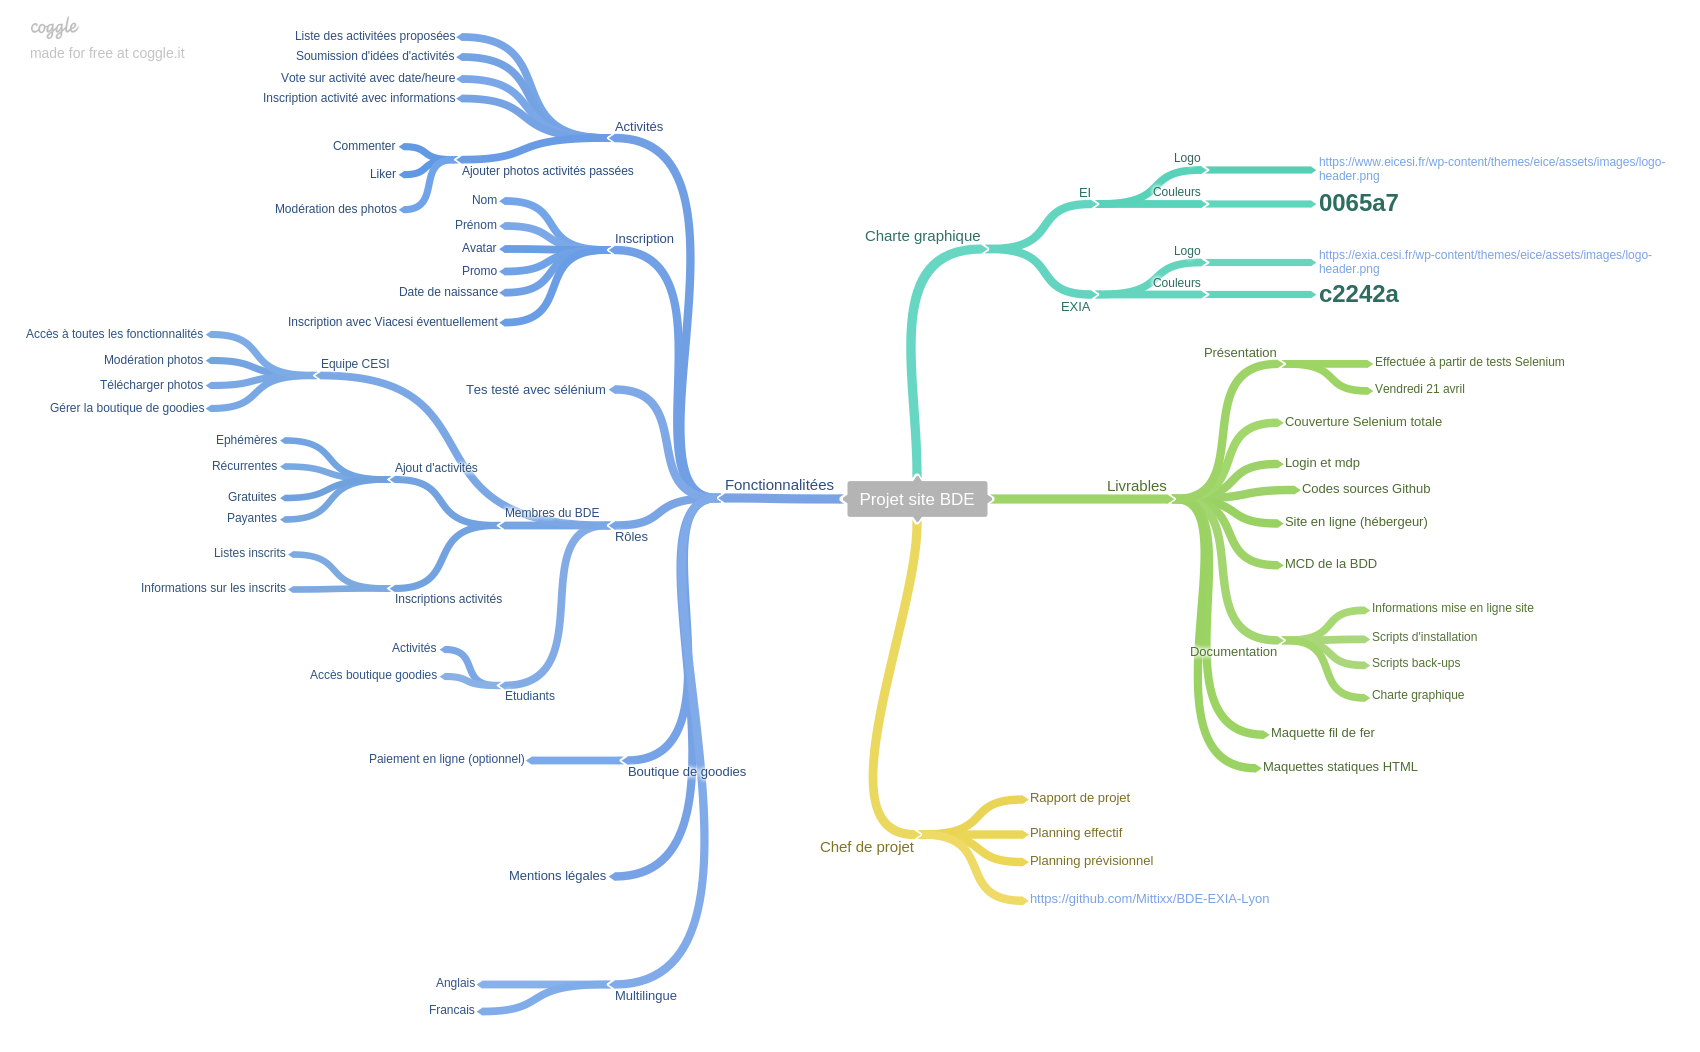
\includegraphics[scale=0.25]{img/Projet_site_BDE.png}
				\caption{Mind map of the project}
			\end{figure}

			This tool help us to have a clear understanding of the website and to be sure not to pass next to important features. A full-width version of this mind map is available on the github repository\footnote{https://github.com/Mittixx/BDE-EXIA-Lyon}.

			\paragraph{Balsamiq}
				We used this software to create the wireframe of the website, it is very simple drag-and-drop system with pre-built widgets. All the wireframe are available at this url \href{https://github.com/Mittixx/BDE-EXIA-Lyon/tree/master/Mockup/Balsamiq}{https://github.com/Mittixx/BDE-EXIA-Lyon/tree/master/Mockup/Balsamiq}. An exemple of wireframe : 	
				\begin{figure}[h]
					\centering
					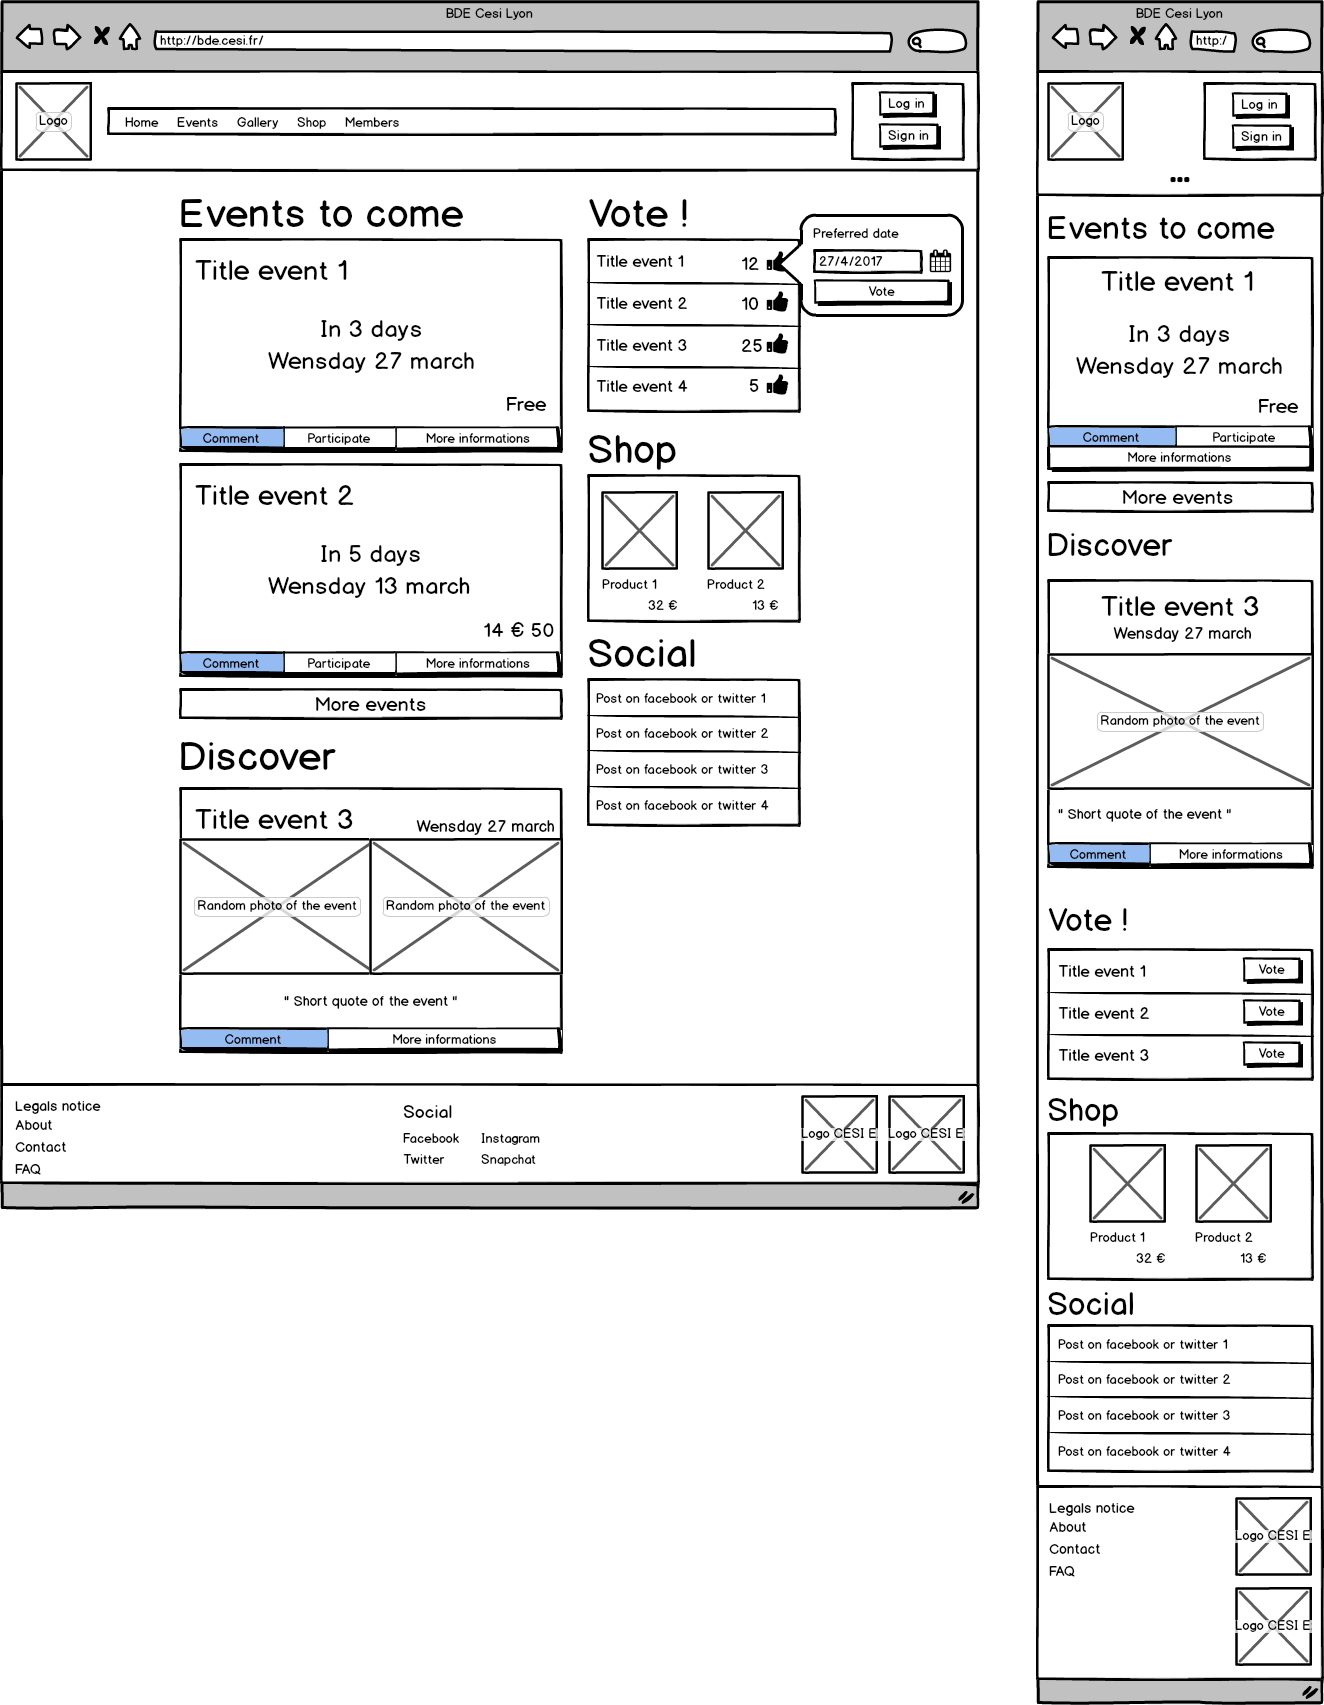
\includegraphics[scale=0.25]{img/balsamiq-wireframe-home.png}
					\caption{Homepage wireframe created with Balsamiq}
				\end{figure}
				
			
			\paragraph{Git}
				Of course we used the version control system Git to track changes and to coordinate the work on the files, to build the website but also this report. The link of the github repository is at the bottom of this page (footnote).

			\paragraph{}
				To developp we used two code editor : \textbf{Sublime Text} and \textbf{PHPStorm}, two excellent code editor to help us through the development of the website. We also used several tools, as \textbf{Docker} to have a container for the servers, \textbf{Xdebug} to have a full debuging tool with the ability to use breakpoint, \textbf{Latex} to create collaboratively this report and \textbf{Draw.io} to easily create diagram.

				\paragraph{Symfony}
					We made the choice to use the framework Symfony to facilitate the development of the website backend. It allowed us to gain time on the creation of CRUDs function, the creation of entity and the integration of the entity in the template.
